% !TEX encoding = UTF-8 Unicode
%%==================================================
%% thanks.tex for SJTU Bachelor Thesis
%% version: 0.5.2
%% Encoding: UTF-8
%%==================================================

\chapter{Hidden Markov Models}
\label{chap:HMM}

In this chapter we formally introduce the hidden Markov models (HMM).
In Sec.\,\ref{sec:HMM:overview} we examine the structure of HMM and 
some fundamental but significant statistics.
A brief introduction to the history of HMM is also covered.
The core part of this chapter lies in Sec.\,\ref{sec:HMM:EM},
i.e.\,how to estimate the model parameters for further analysis and predictions 
with the so-called Baum-Welch or Expectation Maximization (EM) algorithm.
Principles and derivations are explained in details, 
and every module and step of the algorithm is specified.
Sec.\,\ref{sec:HMM:predeco} firstly introduces the method to forecast the series 
based on model parameters deduced with the algorithm.
Then we discuss about techniques to analyze the behavior of the hidden states,
which is known as decoding.

%%%%%%%%%%%%%%%%%%%%%%%%%%

\section{Model overview}
\label{sec:HMM:overview}
As is apparently indicated in its name, 
a hidden Markov model (HMM) is closely related to Markov chains but
with additional existence of latent elements.
Generally speaking, a HMM is a doubly stochastic process \cite{Rabiner:1986jk}.
One stochastic process cannot be directly observed while
the other sequence is observable,
of which the probability distribution of the observed variable is 
conditional on the hidden states,
i.e.\,the underlying and unobserved process.
Specifically, the underlying process is considered to satisfy the Markovian property
and HMM is thus named.
HMM is also known as `hidden Markov process' \cite{Ephraim:2002ju},
`Markov-dependent mixture' \cite{Leroux:1992ma},
`Markov-switching model' \cite{Haas:2004ek},
`Markov mixture model' or `models subject to Markov regime' \cite{Zucchini:2009df},
and these are just different names of HMM.

The model was firstly proposed by Ruslan L.~Stratonovich in \cite{Stratonovich:1960vh},
who also firstly propose the forward-backward procedure (see Sec.\,\ref{sec:HMM:EM:fwdbwd}).
As we described in Sec.\,\ref{sec:preliminary:markov},
states in a typical Markov chain are observable,
thus the only parameters need estimating are the state transition probabilities (matrix).
In a HMM, one of the two series is visible and 
each output is distributed conditional on the hidden states.
The hidden states are distributed in a potential set with corresponding symbols.
The directly observed sequence and the sequence of state symbols 
(which might need to be deduced from the observations)
together provide information about the model.

HMM, due to its probabilistic property, 
is considered as the simplest form of a dynamic Bayesian network \cite{wiki:hmm}.
Besides its application in the financial industry (see Sec.\,\ref{sec:introduction:background}),
the model is mainly applied to pattern recognition 
such as speech recognition and part-of-speech tagging \cite{wiki:hmm,Rabiner:1989hs},
and bioinfomatics like health trajectory \cite{Ghassempour:2014ew}.

In more general HMMs,
the latent variable is not limited to the form of hidden states represented with tokens.
The latent variables themselves could be mathematically meaningful,
either discrete or continuous.
We will cover this part in Sec.\,\ref{sec:future:PF}.
Currently in this section, we only deal with hidden states that are categorical.


\subsection{Model formulation}
\label{sec:HMM:overview:formulation}

        \begin{figure}[!hbt]
        \center
        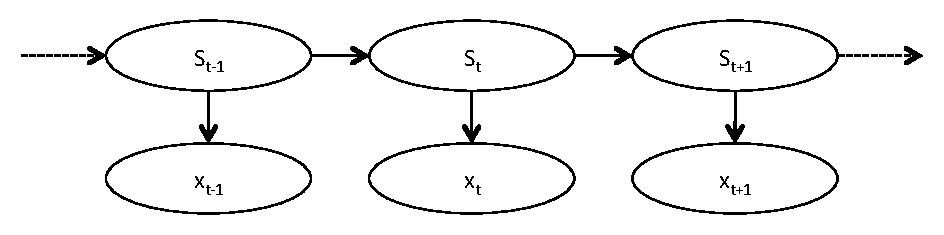
\includegraphics[width=\textwidth]{HMM.pdf}
        \caption{Directed graph of a typical HMM}
        \label{fig:HMM:overview}
        \end{figure}
Illus.\,\ref{fig:HMM:overview} plots a typical HMM in the simplest way.
The model is within the area dependent mixture models,
with $S_t$ representing the hidden states process and 
$X_t$ representing the observed variable,
i.e.\,the visible realizations of the other stochastic process.

The hidden states process $\{S_t \colon t = 1,2,\dots\}$ is a Markov chain: 
        \begin{equation}
        \label{eq:HMM:states}
        \prob{S_t \mid \bS^{(t-1)}} = \prob{S_t \mid S_{t-1}},\ t = 2,3,\dots,
        \end{equation}
and the observed variable has a probability distribution
conditional only on the current hidden state:
        \begin{equation}
        \label{eq:HMM:prob}
        \prob{X_t \mid \bX^{(t-1)}, \bS^{(t-1)}} = \prob{X_t \mid S_t},\ t = 1,2,3,\dots.
        \end{equation}
Values of the hidden states are categorical tokens that qualitatively distinguishes the states.
The number of symbols in the feasible set defines the name of the HMM,
e.g.\,if there are in total $N$ possible hidden states,
the model is then referred to as a $N$-state HMM.
The transition of each state from and to one another 
is exactly the same as one shown in Illus.\,\ref{fig:markov:transition}

The probability $\prob{X_t \mid S_t}$ in Eq.\,\ref{eq:HMM:prob} 
can be used to derive the probability mass/density functions for discrete/continuous observations.
We introduce the notation $p_i$, for $i = 1,2,\dots,N$, where
		\begin{equation}
        \label{eq:HMM:distribution}
        p_i(x) = \left \{ 
        \begin{array}{l l}
        \prob{X_t = x \mid S_t = i} & ,\text{if}\ X_t\ \text{is discrete,} \\
        f_t(x \mid S_t = i) & ,\text{if}\ X_t\ \text{is continuous.} \\
        \end{array} \right.
        \end{equation}
We refer to the $N$ distributions $\{p_i\}_{i=1}^{N}$ as state-dependent distribution, 
or simply conditional distributions, 
since the probability distributions are conditional on the states.
The distributions are irrelevant with time $t$ owing to their time homogeneity.
In the following sections,
we merely consider the case where $X_t$ is discrete,
as the observed stock return series that will be discussed about 
in Ch.\,\ref{chap:system} and \ref{chap:positive} are discretely sampled.


\subsection{Marginal distributions}
\label{sec:HMM:overview:distribution}
With knowledge of Markov chain (Sec.\,\ref{sec:preliminary:markov}) and 
Eq.\,\ref{eq:HMM:states},\ref{eq:HMM:prob} and \ref{eq:HMM:distribution},
we are able to find the marginal distributions of the observed series $X_t$.


Consider the marginal probability
		\begin{equation}
		\label{eq:HMM:marginal}
		\begin{aligned}
		\prob{X_t = x} & = \sum_{i=1}^{N} \prob{X_t = x \mid S_t = i}\prob{S_t = i} \\
		& = \sum_{i=1}^N p_i(x)\delta_i(t).
        \end{aligned}
        \end{equation}
We can rewrite Eq.\,\ref{eq:HMM:marginal} in form of matrix:

		\begin{equation}
		\label{eq:HMM:marginalmat}
		\begin{aligned}
		\prob{X_t = x} & = (\delta_1(t),\delta_2(t),\dots,\delta_N(t)) 
			\left ( \begin{array} {c c c}
				p_1(x) & & 0 \\
				& \ddots & \\
				0 & & p_N(x) \\
			\end{array} \right)
			\left ( \begin{array} {c}
				1 \\	\vdots \\	1 \\
			\end{array} \right) \\
		& = \bdelta(t)\bp(x)\one,
        \end{aligned}
        \end{equation}
where $\bp(x)$ is the diagonalized matrix of $(p_1(t),p_2(t),\dots,p_N(t))$.

Since $\bdelta(t) = \bpi\bGamma^{t-1}$ (Eq.\,\ref{eq:preliminary:markov:unconditional}), 
we shall rewrite Eq.\,\ref{eq:HMM:marginalmat} as 
		\begin{equation}
		\label{eq:HMM:marginalmatsimple}
		\prob{X_t = x} = \bpi\bGamma^{t-1}\bp(x)\one.
        \end{equation}

We also care about the bivariate distribution of $X_t$.
Firstly we consider the joint probability expressed in conditional probabilities:
		\begin{equation}
		\label{eq:HMM:joint}
		\prob{X_t,X_{t+k},S_t,S_{t+k}} = 
			\prob{S_t}\prob{X_t \mid S_t}\prob{S_{t+k} \mid S_t}\prob{X_{t+k} \mid S_{t+k}},
        \end{equation}
which leads to
		\begin{equation}
		\label{eq:HMM:bivariate}
		\begin{aligned}
		\prob{X_t = v,X_{t+k} = w} & = 
			\sum_{i=1}^{N}\sum_{j=1}^{N} \prob{X_t = v,X_{t+k} = w,S_t = i,S_{t+k} = j} \\
		& = \sum_{i=1}^{N}\sum_{j=1}^{N} 
			\prob{S_t = i}p_i(v)\prob{S_{t+k} = j \mid S_t = i}p_j(w) \\
		& = \sum_{i=1}^{N}\sum_{j=1}^{N} \delta_i(t)p_i(v)\gamma_{ij}(k)p_j(w) \\
		& = \bdelta(t)\bp(v)\bGamma^k\bp(w)\one.
        \end{aligned}
        \end{equation}

Thus, we can derive the expectation of $X_t$:
		\begin{equation}
		\label{eq:HMM:expectation}
		E(X_t) = \sum_{i=1}^{N} \delta_i(t)E(X_t \mid S_t = i).
		\end{equation}
Eq.\,\ref{eq:HMM:expectation} plays an important role in 
the series prediction that will be talked about later.

\subsection{The likelihood}
\label{sec:HMM:overview:likelihood}
One of the most important statistics of a statistical model is its (log) likelihood.
Therefore, we present a practical way to compute the likelihood $L_T$
of the $N$-state HMM given observations $\{x_t \colon t = 1,2,\dots,T\}$.
With knowledge of the likelihood,
we shall estimate the model parameters through numerical maximization of the likelihood
or other methods that require computable likelihood.

Consider a $N$-state HMM with initial distribution $\bpi$, 
transition matrix $\bGamma$,
and diagonalized conditional probability density functions $p_i$.
The explicit form of the likelihood is then given by
		\begin{equation}
		\label{eq:HMM:likelihood}
		L_T = \bpi\bp(x_1)\bGamma\bp(x_2)\bGamma\bp(x_3)\cdots\bGamma\bp(x_T)\one.
		\end{equation}
The result is quite elegant and we omit the derivation here,
as it is not the main concern of this work.
The reader shall refer to \cite{Zucchini:2009df} for the proof of this conclusion.
The reader should also notice that \cite{Zucchini:2009df} provides details about the likelihood
when observation data are missing at random or interval-censored.
Corresponding adjustments should be taken to properly calculate the likelihood.
Since the empirical analysis data that we will use in Ch.\,\ref{chap:positive} 
are required to be complete and tidy,
we avoid unnecessary explanations for these cases in this thesis.

%%%%%%%%%%%%%%%%%%%%%%%%%%

\section{Model estimation with Expectation Maximization algorithm}
\label{sec:HMM:EM}
Knowing how to compute the likelihood of a HMM, 
we can estimate the model parameters by direct maximization of the likelihood,
i.e.\,fulfill the task of model estimation with MLEs.
Another commonly implemented method is the so-called Expectation Maximization (EM) algorithm.

The EM algorithm is specifically known as Baum-Welch algorithm within the area of HMMs,
and the method is firstly proposed in \cite{Baum:1966cy,Baum:1967gs,Baum:1970do}.
The algorithm deals with Markovian hidden states series 
that is homogeneous but not necessarily stationary.
Apart from the state transition matrix,
the initial distribution $\bpi$ is also estimated and 
so is the conditional distribution probability density function.
We will first introduce the forward and backward procedure in Sec.\,\ref{sec:HMM:EM:fwdbwd}
and then present the full version of EM in Sec.\,\ref{sec:HMM:EM:algo}.


\subsection{Forward and backward procedure}
\label{sec:HMM:EM:fwdbwd}
Recall Eq.\,\ref{eq:HMM:likelihood} for the form of likelihood:
		\begin{equation*}
		\label{eq:HMM:likelihood2}
		L_T = \bpi\bp(x_1)\bGamma\bp(x_2)\bGamma\bp(x_3)\cdots\bGamma\bp(x_T)\one,
		\end{equation*}
and we provide the definitions of forward and backward probabilities as follows.
		
		\begin{defn}
		\label{defn:fwd}
		For $t = 1,2,\dots,T$, define the row vector $\balpha_t$ as
			\begin{equation}
			\label{eq:HMM:fwd:defn}
			\balpha_t = \bpi\bp(x_1)\bGamma\bp(x_2)\bGamma\bp(x_3)\cdots\bGamma\bp(x_t)
			 = \bpi\bp(x_1)\prod_{s=2}^{t}\bGamma\bp(x_s),
			\end{equation}
		and refer to the elements as forward probabilities.
		\end{defn}

		\begin{defn}
		\label{defn:bwd}
		For $t = 1,2,\dots,T$, define the row vector $\bbeta_t$ as
			\begin{equation}
			\label{eq:HMM:bwd:defn}
			\bbeta_t = \bGamma\bp(x_{t+1})\bGamma\bp(x_{t+2})\cdots\bGamma\bp(x_T)\one
			 = \left(\prod_{s=t+1}^{T}\bGamma\bp(x_s)\right)\one,
			\end{equation}
		and refer to the elements as backward probabilities. 
		The case $t = T$ yields $\bbeta_T = 1$.
		\end{defn}

It is easy to find that we can rewrite Eq.\,\ref{eq:HMM:fwd:defn} in the form of recursion that 
for $t = 1,2,\dots,T-1, \balpha_{t+1} = \balpha_t\bGamma\bp(x_{t+1})$.
With derivation based on Bayesian formula 
(similar to \ref{eq:HMM:likelihood},see \cite{Zucchini:2009df}),
we have the following proposition:

		\begin{prop}
		\label{prop:fwd}
		For $t = 1,2,\dots,T$ and $j = 1,2,\dots,N$,
			\begin{equation}
			\label{eq:HMM:fwd:prop}
			\alpha_t(j) = \prob{\bX^{(t)} = \bx^{(t)}, S_t = j}.
			\end{equation}
		The element $\alpha_t(j)$ is thus called the forward probability.
		\end{prop}

Similarly, we can rewrite Eq.\,\ref{eq:HMM:bwd:defn} as that 
for $t = 1,2,\dots,T-1, \bbeta_{t}^{\prime} = \bGamma\bp(x_{t+1})\bbeta_{t+1}^{\prime}$,
and suggest the similar proposition:
	
		\begin{prop}
		\label{prop:bwd}
		For $t = 1,2,\dots,T-1$ and $i = 1,2,\dots,N$,
			\begin{equation}
			\label{eq:HMM:bwd:prop}
			\beta_t(i) = \prob{\bX^{(t+1:T)} = \bx^{(t+1:T)} \mid S_t = i},\ \prob{S_t = i}>0.
			\end{equation}
		The element $\beta_t(i)$ is thus called the backward probability.
		\end{prop}
Note that the forward probabilities are joint probabilities while
backward probabilities are conditional probabilities.

With Eq.\,\ref{eq:HMM:likelihood},\ref{eq:HMM:fwd:prop} and \ref{eq:HMM:bwd:prop},
we can rewrite the likelihood with forward and backward probabilities:
		\begin{equation}
		\label{eq:HMM:likelihood:fwdbwd}
		\alpha_t(i)\beta_t(i) = \prob{\bX^{(T)} = \bx^{(T)}, S_t = i} \LRa
		L_T = \prob{\bX^{(T)} = \bx^{(T)}} = \balpha_t\bbeta_t^{\prime}.
		\end{equation}
The equation can be easily proved with Def.\,\ref{defn:fwd} and \ref{defn:bwd} 
and we omit the derivation here.

In order to apply the results to the EM algorithm,
we also need the conditional probabilities of the hidden states given observations.
	
		\begin{prop}
		\label{prop:states}
		For $t = 1,2,\dots,T$,
			\begin{equation}
			\label{eq:HMM:states:cond}
			\prob{S_t = j \mid \bX^{(T)} = \bx^{(T)}} = \frac{\alpha_t(j)\beta_t(j)}{L_T},
			\end{equation}
		and for $t = 2,\dots,T$,
			\begin{equation}
			\label{eq:HMM:states:trans}
			\prob{S_{t-1} = j,S_t = k \mid \bX^{(T)} = \bx^{(T)}} = 
			\frac{\alpha_{t-1}(j)\gamma_{jk}p_k(x_t)\beta_t(k)}{L_T},
			\end{equation}
		\end{prop}
Results in Prop.\,\ref{prop:states} will be applied in both model estimation and decoding.


\subsection{The EM algorithm}
\label{sec:HMM:EM:algo}
The traditional EM algorithm iteratively maximize the likelihood of the model
and to find the MLEs under circumstances of missing data.
Baum-Welch algorithm refers to this idea and consider the sequence of hidden states
as missing data since they are unobserved.

We denote the model parameters as $\btheta$ and try to compute the 
complete-data log-likelihood (CDLL),
i.e.\,the log-likelihood of parameters $\btheta$.
Then EM can be carried out by two steps:
		\begin{itemize}
		\item \textbf{E step} calculates the expectations of (functions of) the missing data 
		conditional on the observations and the current estimate of $\btheta$.
		\item \textbf{M step} maximizes the CDLL w.r.t.\,$\btheta$.
		\end{itemize}
The iteration carries on until convergence,
and the final $\btheta$ is the stationary point of the likelihood,
which is the model parameter set that we want to figure out.

We define two indicators, of which the value is either zero or one.
		\begin{equation}
		\label{eq:HMM:EM:indicator}
		u_j(t) = \left \{ \begin{array}{l l}
		1 & ,\text{iff}\ S_t = j \\
		0 & ,\text{otherwise}, \\
		\end{array} \right.
		\text{and}\quad
		v_{jk}(t) = \left \{ \begin{array}{l l}
		1 & ,\text{iff}\ S_{t-1} = j\ \text{and}\ S_t = k \\
		0 & ,\text{otherwise}. \\
		\end{array} \right.
		\end{equation}
Then we rewrite the likelihood of HMM,
viewing hidden states $S_1,S_2,\dots,S_T$ as missing data,
in terms of the indicators and parameters:
		\begin{equation}
		\label{eq:HMM:EM:CDLL}
		\log\left(\prob{\bx^{(T)},\bs^{(T)}}\right) = 
		\underbrace{\sum_{j=1}^{N} u_j(1)\log\pi_j}_{\text{term 1}} + 
		\underbrace{\sum_{j=1}^{N}\sum_{k=1}^{N} \left(\sum_{t=2}^Tv_{jk}(t)\right)\log\gamma_{jk}}
			_{\text{term 2}} + 
		\underbrace{\sum_{j=1}^{N}\sum_{t=1}^{T} u_j(t)\log p_j(x_t)}_{\text{term 3}}.
        \end{equation}
Iterative maximization of the CDLL will provide us information about 
both $\bpi$, the initial distribution and $\bGamma$, the state transition matrix.

Apply Eq.\,\ref{eq:HMM:EM:CDLL} to the general EM and we can specify the two steps as
		\begin{itemize}
		\item \textbf{E step} replaces the two indicator vectors by their conditional expectations
		given observations $\bx^{(T)}$ and the current parameter estimates
			\begin{subequations}
			\begin{align}
			\label{eq:HMM:EM:ind_u}
			\hat{u}_j(t) & = \prob{S_t = j \mid \bx^{(T)}} = \frac{\alpha_t(j)\beta_t(j)}{L_T},\\
			\label{eq:HMM:EM:ind_v}
			\hat{v}_{jk}(t) & = \prob{S_{t-1} = j,S_t = k \mid \bx^{(T)}} = 
				\frac{\alpha_{t-1}(j)\gamma_{jk}p_k(x_t)\beta_t(k)}{L_T}.
			\end{align}
			\end{subequations}
		\item \textbf{M step} maximizes the CDLL, Eq.\,\ref{eq:HMM:EM:CDLL},
		w.r.t.\,the initial distribution $\bpi$, the state transition matrix $\bGamma$,
		and conditional distribution parameters which is embedded in $p_j(x_t)$ in term 3.
		\end{itemize}

Notice that we have split the computation of CDLL into three terms 
so that the maximizations w.r.t.\,the three parameter sets are independent.
Furthermore, the separation guarantees the existence of analytic solutions.
We present the sub-problems and corresponding solutions as follows.

\subsubsection{Initial distribution}
\label{sec:HMM:EM:algo:initial}
By term 1 in Eq.\,\ref{eq:HMM:EM:CDLL}, consider the maximization problem
		\begin{equation}
		\label{eq:HMM:EM:max:1}
		\max_{\bpi} \sum_{j=1}^{N} u_j(1)\log\pi_j,
		\end{equation}
and the solution is given as
		\begin{equation}
		\label{eq:HMM:EM:sol:1}
		\pi_j = \frac{\hat{u}_j(1)}{\sum_{j=1}^{N}\hat{u}_j(1)} = \hat{u}_j(1).
		\end{equation}


\subsubsection{State transition matrix}
\label{sec:HMM:EM:algo:transition}
By term 2 in Eq.\,\ref{eq:HMM:EM:CDLL}, consider the maximization problem
		\begin{equation}
		\label{eq:HMM:EM:max:2}
		\max_{\bGamma} \sum_{j=1}^{N}\sum_{k=1}^{N} \left(\sum_{t=2}^Tv_{jk}(t)\right)\log\gamma_{jk},
		\end{equation}
and the solution is given as
		\begin{equation}
		\label{eq:HMM:EM:sol:2}
		\begin{aligned}
		\gamma_{jk} & = \frac{f_{jk}}{\sum_{k=1}^{N} f_{jk}}, \\
		\text{where}\quad f_{jk} & = \sum_{t=2}^{T} \hat{v}_{jk}(t).
		\end{aligned}
		\end{equation}


\subsubsection{Conditional distribution}
\label{sec:HMM:EM:algo:distribution}
By term 3 in Eq.\,\ref{eq:HMM:EM:CDLL}, consider the maximization problem
		\begin{equation}
		\label{eq:HMM:EM:max:3}
		\max_{\btheta} \sum_{j=1}^{N}\sum_{t=1}^{T} u_j(t)\log p_j(x_t;\btheta).
		\end{equation}
The solution to this sub-problem depends on the formulation of the conditional distribution,
and is deduced through common MLE method.
We provide solutions to two kind of distributions here,
one for Poisson and the other for normal.

For Poisson distributions we have $p_j(x) = e^{-\lambda_j}\frac{\lambda_j^x}{x!}$,
the solution is then given as 
		\begin{equation}
		\label{eq:HMM:EM:sol:3:poisson}
		\hat{\lambda}_j = \frac{\sum_{t=1}^{T} \hat{u}_j(t)x_t}{\sum_{t=1}^{T} \hat{u}_j(t)}.
		\end{equation}

For normal distributions we have 
$p_j(x) = \frac{1}{\sqrt{2\pi\sigma_j^2}} \exp\{-\frac{(x-\mu_j)^2}{2\sigma_j^2}\}$,
the solution is then given as 
		\begin{subequations}
		\begin{align}
		\label{eq:HMM:EM:sol:3:normal:mu}
		\hat{\mu}_j & = \frac{\sum_{t=1}^{T} \hat{u}_j(t)x_t}{\sum_{t=1}^{T} \hat{u}_j(t)}, \\
		\label{eq:HMM:EM:sol:3:normal:sigma}
		\hat{\sigma}_j & = \frac{\sum_{t=1}^{T} \hat{u}_j(t)(x_t - \hat{\mu}_j)^2}
							  {\sum_{t=1}^{T} \hat{u}_j(t)}.
		\end{align}
		\end{subequations}
The results above are thus easy to compute and can be 
directly applied in the numerical realization procedures.

%%%%%%%%%%%%%%%%%%%%%%%%%%

\section{Prediction and decoding}
\label{sec:HMM:predeco}
The series prediction is essentially an application of the forecast distributions.
With model parameters estimated,
we can fulfill the prediction by one-step or multiple-step forecast.
We cover this topic in Sec.\,\ref{sec:HMM:predeco:forecast}.

Information of the historical hidden states distributions can be also deduced.
The process of find the states occupied by the Markov chain is referred to as decoding,
Decoding can be further classified as local ones and global ones
in terms of the likelihood to be maximized.
Both decoding procedures are discussed in this section.
Specifically, we introduce the Viterbi algorithm that is implemented for global decoding 
in Sec.\,\ref{sec:HMM:predeco:glodeco}.


\subsection{Forecast distributions}
\label{sec:HMM:predeco:forecast}
Consider $h$-step forecast distribution conditional on the observations
		\begin{equation}
		\label{eq:HMM:predeco:forecast}
		\begin{aligned}
		\prob{X_{T+h} = x \mid \bX^{(T)} = \bx^{(T)}} & = 
			\frac{\prob{\bX^{(T)} = \bx^{(T)}, X_{T+h} = x}}{\prob{\bX^{(T)} = \bx^{(T)}}} \\
		& = \frac{\balpha_T\bGamma^h\bp(x)\one}{\balpha_T\one}. 
		\end{aligned}
		\end{equation}
In order to perform one-step prediction,
we can simply assign $h$ with value one and obtain the result.

Notice that when $h$ increases, 
the result stated in Eq.\,\ref{eq:HMM:predeco:forecast} will converge
due to the convergence of Markov chain state transition matrix, i.e.
		\begin{equation}
		\label{eq:HMM:predeco:forecast:converge}
		\lim_{h\ra\infty}\prob{X_{T+h} = x \mid \bX^{(T)} = \bx^{(T)}} = \bdelta^{\ast}\bp(x)\one,
		\end{equation}
where $\bdelta^{\ast}$ represents the stationary distribution of the Markov chain
(see Sec.\,\ref{sec:preliminary:markov:stationary}).
One of the direct influences of the convergence is that
we cannot take a too big $h$ in our stock return series prediction system,
or the prediction results would be smoothed due to the converging property.


\subsection{State probabilities and local decoding}
\label{sec:HMM:predeco:locdeco}
The concept of decoding is firstly adopted in speech recognition areas \cite{Fredkin:1992ba},
and, in the context of HMM,
refers to the procedure to find the most probable sequence of hidden states
that generates the observation series.
The idea `local decoding' of the state at a specific time 
stands for the determination of the most possible state at that time node.

Recall Eq.\,\ref{eq:HMM:states:cond}
		\begin{equation*}
		\prob{S_t = j \mid \bX^{(T)} = \bx^{(T)}} = \frac{\alpha_t(j)\beta_t(j)}{L_T},
		\end{equation*}
we are able to compute the likelihood $L_T$ with EM algorithm,
and therefore able to calculate the state probabilities and 
decide the most probable state at each $t$:
		\begin{equation}
		\label{eq:HMM:predeco:locdeco:state}
		S_t^{\ast} = \argmax_{j = 1,2,\dots,N} \prob{S_t = j \mid \bX^{(T)} = \bx^{(T)}}.
		\end{equation}


\subsection{Global decoding and Viterbi algorithm}
\label{sec:HMM:predeco:glodeco}
Local decoding only provides information of the most probable state for each separate time $t$
but tells nothing about the most likely sequence of the states over the entire period.
Global decoding solves a slightly different maximization problem as local decoding,
and the result is often similar but not exactly identical.

The global decoding procedure enables us to find 
the conditional probability of the entire hidden state series given the observations, i.e.
		\begin{equation}
		\label{eq:HMM:predeco:glodeco:prob}
		\prob{\bS^{(T)} = \bs^{(T)} \mid \bX^{(T)} = \bx^{(T)}}.
		\end{equation}

The maximization problem can be solved with an algorithm named after Viterbi \cite{Viterbi:1967hq},
which is a very effective dynamic programming technique.
Define the probabilities $\xi_{ti}$ as follows:
		\begin{equation}
		\label{eq:HMM:predeco:viterbi:defn}
		\begin{aligned}
		\xi_{1i} & = \prob{S_1 = i,X_1 = x_1} = \pi_ip_i(x_1), \\
		\xi_{ti} & = \max_{s_1,s_2,\dots,s_{t-1}} 
			\prob{\bS^{(t-1)} = \bs^{(t-1)},S_t = i, \bX^{(T)} = \bx^{(T)}},
		\end{aligned}
		\end{equation}
for $t = 2,3,\dots,T$.
We can also rewrite Eq.\,\ref{eq:HMM:predeco:viterbi:defn} in a recursive form:
		\begin{equation}
		\label{eq:HMM:predeco:viterbi:defn_2}
		\begin{aligned}
		\xi_{1i} & = \prob{S_1 = i,X_1 = x_1} = \pi_ip_i(x_1), \\
		\xi_{tj} & = \left(\max_i(\xi_{t-1,i}\gamma_{ij})\right)p_j(x_t),
		\end{aligned}
		\end{equation}
for $t = 2,3,\dots,T$ and $i = 1,2,\dots,N$.
The $T\times N$ matrix enables us to solve the maximization problem with 
computational complexity that is linear in $T$.
The result can be solved recursively from:
		\begin{equation}
		\label{eq:HMM:predeco:viterbi:defn_3}
		\begin{aligned}
		S_T & = \argmax_{i = 1,2,\dots,N} \xi_{Ti}, \\
		S_t & = \argmax_{i = 1,2,\dots,N} (\xi_{ti}\gamma_{i,S_{t+1}}),
		\end{aligned}
		\end{equation}
for $t = T-1, T-2,\dots,1$.

The maximization can also be rewritten in form of logarithms,
and scaling problems should be noticed to avoid numerical underflows.
This problem is explained in \cite{Zucchini:2009df} with details.




